% Chapter Template

\chapter{Ensayos y resultados} % Main chapter title

\label{Chapter4} % Change X to a consecutive number; for referencing this chapter elsewhere, use \ref{ChapterX}
En este capítulo se describe el conjunto de ensayos realizados sobre el sistema y se recopilan sus resultados.
Con este propósito, se explican las características del \textit{hardware} y el banco de pruebas que se emplearon.
Además, se explican los criterios de evaluación para determinar la calidad de las respuestas de los
modelos extensos de lenguaje.
Finalmente, se hace un análisis global de los resultados, destacando el grado de mejora que ofrece el sistema, así como
sus errores más comunes.

%----------------------------------------------------------------------------------------
%	SECTION 1
%----------------------------------------------------------------------------------------

\section{Entorno y banco de pruebas}
Los ensayos fueron ejecutados en un equipo de altas prestaciones, orientado a tareas de cómputo intensivo y procesamiento de modelos de lenguaje de gran tamaño.
Sus especificaciones son las siguientes:
\begin{itemize}
\item Memoria RAM: 64 GB.
\item Tarjeta gráfica: NVIDIA GeForce RTX4080 SUPER, con 16 GB de memoria RAM dedicada.
\item Procesador: AMD Ryzen9 7950X3D 16-Core.
\item Sistema Operativo: Windows 11.
\end{itemize}

Aunque se emplearon diversos \textit{worldbuildings} en el proceso iterativo de refinamiento de las instrucciones,
el contexto narrativo de prueba se basó exclusivamente en textos pertenecientes al mundo de ficción ``Aanrah'',
desarrollado por el autor Necrowmancer en la plataforma de WorldAnvil \cite{aanrah2024}.
Esta ambientación fue seleccionada por ofrecer una combinación equilibrada de complejidad conceptual,
léxico específico y coherencia interna, sin alcanzar un volumen excesivo de contenido.
Dicha elección refleja el tipo de entradas que previsiblemente introducirán los usuarios del sistema,
al tiempo que plantea un desafío suficientemente realista para los modelos extensos de lenguaje.
El corpus de referencia se encuentra detallado en el apéndice \ref{AppendixB}.

%----------------------------------------------------------------------------------------
%	SECTION 2
%----------------------------------------------------------------------------------------

\section{Pruebas de procesamiento de ficheros}
Para comprobar el funcionamiento del procesamiento de los ficheros sin depender del módulo de procesamiento de peticiones \textit{web},
se implementaron varias celdas en un \textit{notebook} de Jupyter.
Esta solución no solo permite evaluar de forma controlada el comportamiento del módulo,
sino que además cumple con los criterios de pruebas automatizadas exigidos por el cliente.

Además, se formateó el contexto narrativo de prueba en los tres tipos de fichero aceptados: txt, docx y pdf.
El funcionamiento del módulo quedó validado tras comprobar que el texto extraído de todos los ficheros es idéntico,
tal y como se muestra en las figuras \ref{fig:txt-read-test}, \ref{fig:docx-read-test} y \ref{fig:pdf-read-test}.
Se aprecian diferencias de formato en el archivo pdf, pero su contenido coincide.

\begin{figure}[htbp]
	\centering
	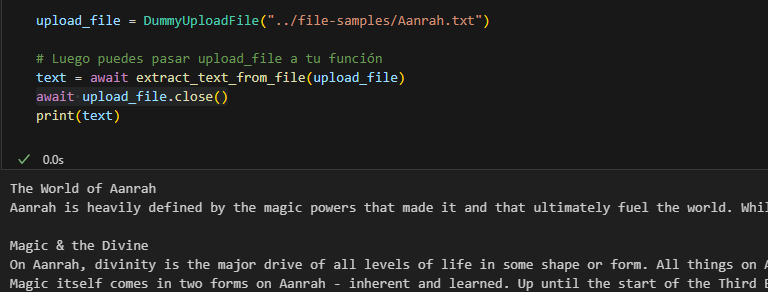
\includegraphics[width=0.9\textwidth]{./Figures/file-read-test-txt.png}
	\caption{Prueba de lectura de ficheros txt.}
	\label{fig:txt-read-test}
\end{figure}

\begin{figure}[htbp]
	\centering
	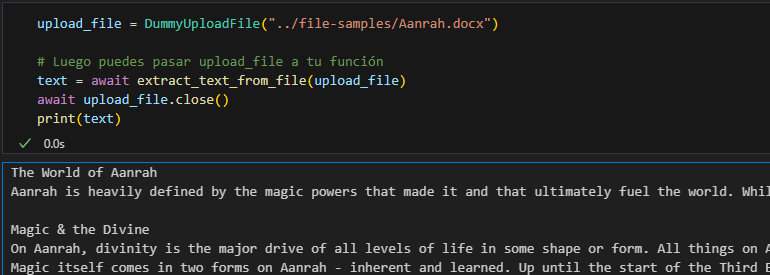
\includegraphics[width=0.9\textwidth]{./Figures/file-read-test-docx.png}
	\caption{Prueba de lectura de ficheros docx.}
	\label{fig:docx-read-test}
\end{figure}

\begin{figure}[htbp]
	\centering
	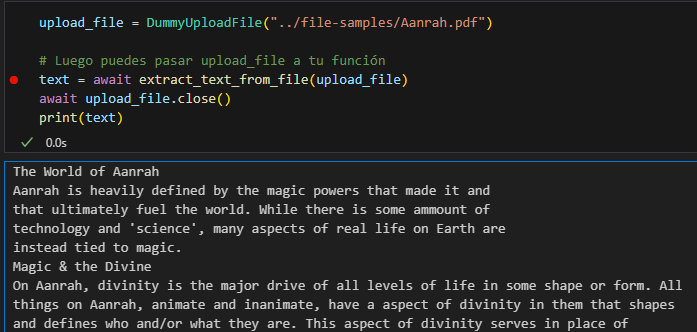
\includegraphics[width=0.9\textwidth]{./Figures/file-read-test-pdf.png}
	\caption{Prueba de lectura de ficheros pdf.}
	\label{fig:pdf-read-test}
\end{figure}

%----------------------------------------------------------------------------------------
%	SECTION 3
%----------------------------------------------------------------------------------------
\pagebreak
\section{Pruebas de procesamiento de peticiones web}
Durante la fase de implementación se llevaron a cabo pruebas incrementales que incluyeron
la verificación de la correcta carga del HTML, la recepción de las peticiones junto con los archivos adjuntos,
la lectura del contenido y, finalmente,
la integración completa del flujo de comunicación entre el usuario y el modelo extenso de lenguaje.
Cuando una petición se procesa correctamente, la información se envía de vuelta a la interfaz \textit{web},
donde se muestra en un cuadro de texto.

En la figura~\ref{fig:web-test} se muestra el resultado de una petición en la que,
con fines de prueba, se omitió el envío al módulo LLM
y en su lugar se devolvió directamente al usuario el contenido del fichero adjunto.

\begin{figure}[htbp]
	\centering
	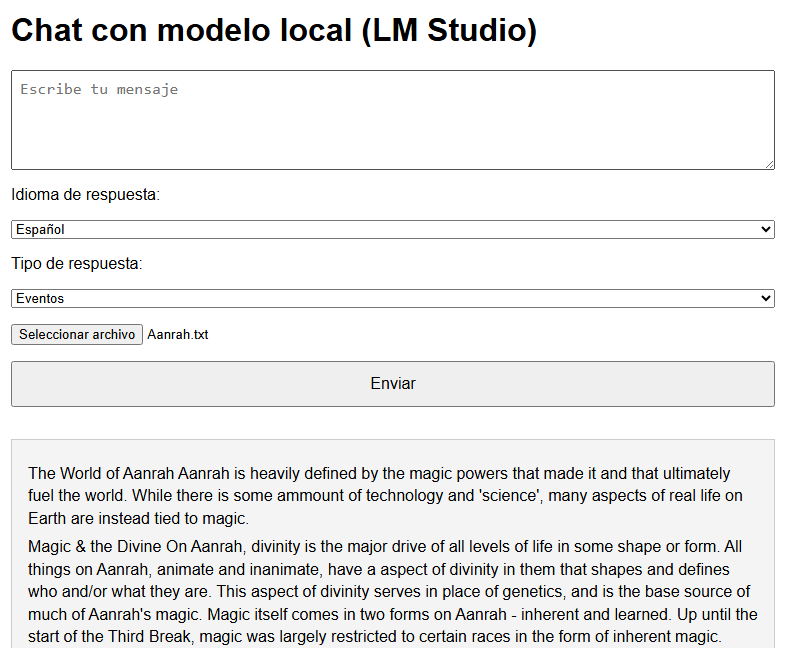
\includegraphics[width=1\textwidth]{./Figures/web-test.png}
	\caption{Prueba de envío de peticiones REST.}
	\label{fig:web-test}
\end{figure}

En las pruebas de los siguientes apartados se muestran múltiples figuras de la interfaz con el flujo completo de datos.

%----------------------------------------------------------------------------------------
%	SECTION 4
%----------------------------------------------------------------------------------------
\section{Método para valorar la salida de los modelos extensos de lenguaje}
En este apartado se explica la lógica que se siguió para valorar la calidad de las respuestas
generadas por el modelo de lenguaje.
Este proceso presenta una dificultad inherente:
debido a la naturaleza de los casos de uso del sistema, esta puntuación es completamente subjetiva.
Conceptos como “adecuación”, “originalidad” o “interés narrativo” no pueden medirse de forma objetiva ni automática,
lo que limita la posibilidad de una evaluación completamente reproducible.
Por ello, la validación fue realizada de forma manual, basándose en mi propio criterio como desarrollador del sistema.

Una vez aclarado este aspecto, las pruebas se estructuraron de forma que pudieran reproducirse de manera sencilla y sistemática.
En todas las evaluaciones se emplea el mismo fichero adjunto, que contiene el contexto narrativo base,
y se combina con cada tipo de elemento de \textit{worldbuilding} que se desea generar.
Este enfoque se aplica de forma consistente a todos los modelos extensos de lenguaje.
Adicionalmente, sobre este mismo conjunto de pruebas se compararán dos escenarios:
uno en el que se utiliza la ingeniería de \textit{prompting} desarrollada en este trabajo,
y otro en el que dicha técnica no se aplica.
Este contraste permitirá evaluar el impacto real de las instrucciones
refinadas sobre los modelos.

Para valorar la salida del modelo se emplearon los siguientes criterios:
\begin{itemize}
\item \textbf{Adecuación contextual}: se verifica que los elementos generados respeten el tono, estilo y detalles del contexto narrativo original.
\item \textbf{Pertinencia temática}: los resultados deben estar alineados con la categoría seleccionada
(por ejemplo, si se ha elegido ``personajes'', la salida no debe incluir ubicaciones o eventos).
\item \textbf{Originalidad}: se valora la capacidad del modelo para proponer ideas nuevas sin repetir explícitamente el contenido del fichero.
\item \textbf{Diversidad}: se analiza si la lista contiene variedad en las propuestas y evita repeticiones o elementos demasiado similares.
\item \textbf{Idioma}: se indica si el modelo acepta texto en español. 
\item \textbf{Consistencia}: analiza la inestabilidad en la respuesta de los modelos,
teniendo en cuenta que todos fueron configurados con una temperatura de 0,7 sobre 1. 
\item \textbf{Errores}: se listan los errores encontrados en las pruebas y se analiza el impacto que tienen.
\end{itemize}

%----------------------------------------------------------------------------------------
%	SECTION 5
%----------------------------------------------------------------------------------------
\section{Pruebas con modelos generalistas y \textit{prompting} poco preciso}
Esta sección analiza el rendimiento de los modelos que no han sido ajustados específicamente
para tareas de ambientación narrativa y que carecen de un refinamiento adecuado en las instrucciones.
El objetivo es simular los resultados que podrían obtenerse si una persona sin experiencia en ingeniería de
\textit{prompting} utilizara las opciones más comunes disponibles en línea.

Para lograr esto, se desactivó el módulo de \textit{prompts} y se bloquearon algunos controles de la interfaz
\textit{web} para que solo aceptara el fichero adjunto, el cuadro de texto y el selector de idiomas.
En la figura \ref{fig:prompt-test} se muestra
cómo el modelo responde libremente a la entrada del usuario.
Una vez validada la funcionalidad, todas las instrucciones se simplificaron en una única frase:
``dame una lista de diez nuevos'' seguido del elemento narrativo que se quería obtener.
\pagebreak
\begin{figure}[htbp]
	\centering
	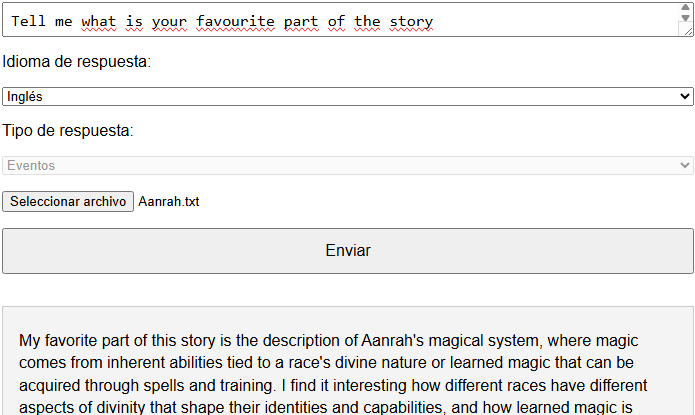
\includegraphics[width=1\textwidth]{./Figures/promp-testing.png}
	\caption{Prueba de desconexión del módulo generador de instrucciones.}
	\label{fig:prompt-test}
\end{figure}

\subsection{Resultados de \textit{deepseek}}
En el caso de \textit{deepseek}, presentó una adaptación al contexto narrativo aceptable y se ciñó correctamente al
tipo de elemento narrativo que se especificó.
No obstante, su desempeño en relación con la variedad de las ideas fue bajo al presentar puntos muy similares entre sí.
Este problema fue especialmente notable en el caso de los personajes y eventos.
Por último, la consistencia de sus respuestas varió en ocasiones.
Esto significa que su sensibilidad a la temperatura es bastante alta.
El modelo puede responder en español, pero los errores de traducción y alucinaciones son frecuentes,
tal y como se muestra en la figura \ref{fig:deepseek-esp}:

\begin{figure}[htbp]
	\centering
	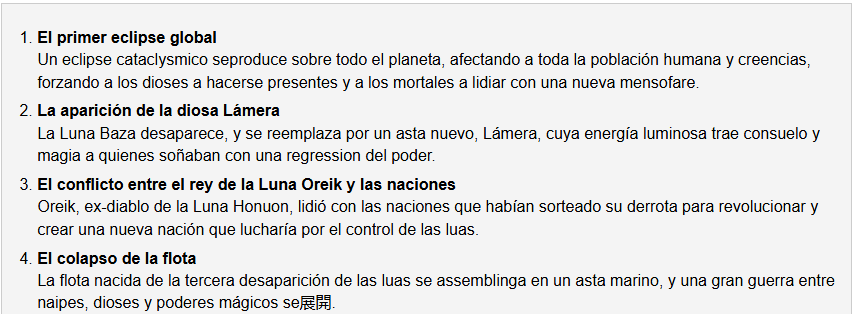
\includegraphics[width=1\textwidth]{./Figures/deepseek-noprompt-spanish.png}
	\caption{Resultado en español de \textit{deepseek} para eventos.}
	\label{fig:deepseek-esp}
\end{figure}
\pagebreak
\subsection{Resultados de \textit{mistral}}
El modelo generalista de \textit{mistral} no consiguió la misma calidad en sus respuestas.
Las propuestas, aunque tienen relación con el contexto de la historia,
muestran una conexión sin demasiada profundidad en los detalles ni en su variedad.
En los casos de geografía y asentamientos, su relación con el contexto es mínima o nula
(ver figura \ref{fig:mistral-geo}), lo que sugiere que su entrenamiento no le permite ser
flexible en la generación de contenido narrativo sin instrucciones previas.
Este modelo pierde completamente el contexto al responder en español,
lo que provoca que utilice referencias reales,
como ciudades de Estados Unidos, personajes históricos o festividades internacionales.

\begin{figure}[htbp]
	\centering
	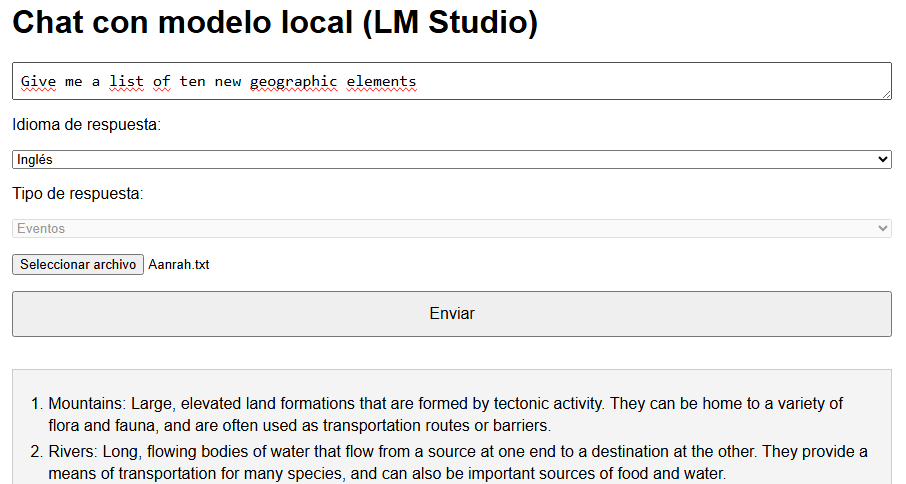
\includegraphics[width=1\textwidth]{./Figures/mistral-noprompt-geography.png}
	\caption{Resultado de \textit{mistral} para geografía}
	\label{fig:mistral-geo}
\end{figure}

%----------------------------------------------------------------------------------------
%	SECTION 6
%----------------------------------------------------------------------------------------
\section{Pruebas con modelos reentrenados y \textit{prompting} poco preciso}
Análogamente a la sección anterior, se llevaron a cabo pruebas equivalentes
sobre los modelos refinados con el fin de evaluar su rendimiento.
Los resultados permiten establecer una comparación entre estos LLM
y los modelos generalistas.

\subsection{Resultados de \textit{writing-roleplay}}
El modelo de \textit{writing-roleplay} funcionó correctamente en la generación de eventos,
comprendiendo adecuadamente el contexto y ofreciendo ideas interesantes.
Sin embargo, presentó problemas en el resto de elementos narrativos.
A pesar de que aporta una variedad aceptable y una ambientación de fantasía correcta,
su respuesta se ajusta más a un contenido predefinido que a algo adaptado a la ambientación
narrativa del fichero adjunto.
Finalmente, fue notoria la inconsistencia del modelo a la temperatura a la que fue configurado,
ya que ocasionalmente repetía información en vez de aportar ideas nuevas.

\subsection{Resultados de \textit{worldbuilder}}
En el caso de \textit{worldbuilder},
su comprensión de la entrada destacó sobre las alternativas generalistas,
aportando ideas con una relación profunda con el contexto de entrada
(Figura \ref{fig:worldbuilder-settle}).
Sin embargo, el modelo también tiene una sensibilidad alta a la temperatura
y ocasionalmente puede ignorar la ambientación al generar nuevo contenido.
Algo único de este LLM es que puede llegar a dar consejos al usuario de cómo
hacer la construcción de mundos, con diversas técnicas y explicaciones,
en vez de dar una lista de nuevas ideas.
También es el único que no puede dar respuestas en español.

\begin{figure}[htbp]
	\centering
	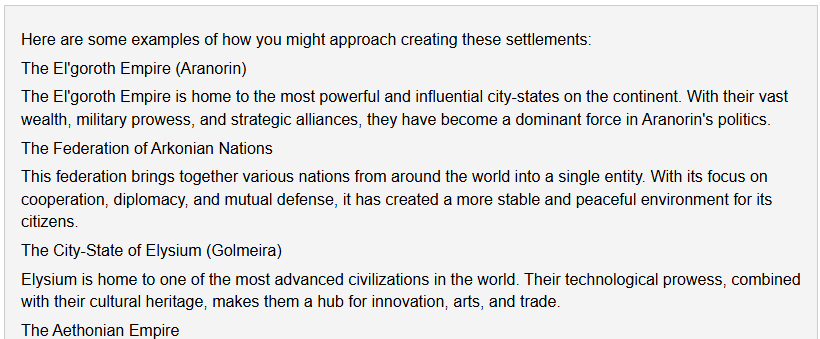
\includegraphics[width=1\textwidth]{./Figures/worldbuilder-noprompt-settlements.png}
	\caption{Resultado de \textit{worldbuilder} para asentamientos}
	\label{fig:worldbuilder-settle}
\end{figure}

\subsection{Resultados de \textit{arliai-rpmax}}
Finalmente, el modelo \textit{arliai-rpmax} fue el que mejor desempeño demostró. 
Se ajustó al contexto de entrada y profundizó en las respuestas de forma aceptable.
Donde también destacó es en la capacidad de generar texto en español sin verse afectado
en la calidad del mensaje. 

A nivel global, todos los LLM funcionaron bien para los eventos y las localizaciones,
mientras que carecieron de originalidad en la generación de personajes y geografía.
En la figura \ref{fig:rpmax-chars} se muestra un ejemplo de este fenómeno.

\begin{figure}[htbp]
	\centering
	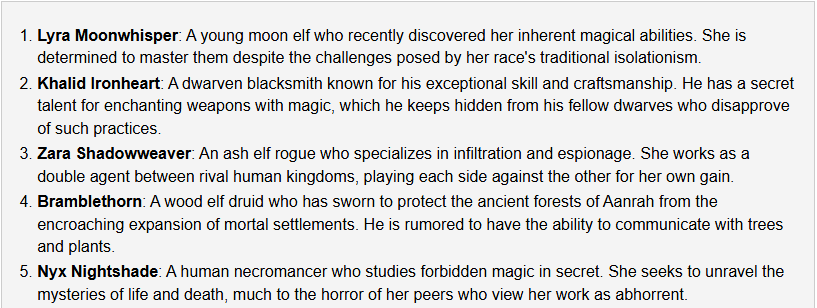
\includegraphics[width=1\textwidth]{./Figures/rpmax-noprompt-chars.png}
	\caption{Resultado de \textit{arliai-rpmax} para personajes}
	\label{fig:rpmax-chars}
\end{figure}

%----------------------------------------------------------------------------------------
%	SECTION 7
%----------------------------------------------------------------------------------------
\section{Pruebas con modelos generalistas y \textit{prompting} preciso}
Esta sección examina el rendimiento de modelos generalistas que no han sido específicamente
ajustados para tareas de ambientación narrativa.
A diferencia de enfoques anteriores sin refinamiento,
el objetivo aquí es maximizar la capacidad intrínseca del modelo mediante instrucciones detalladas,
buscando determinar la eficacia de esta técnica al trabajar con modelos accesibles públicamente.

Para ello, se hace uso del módulo de instrucciones y la interfaz \textit{web}
en su versión final. Tal y como se demuestra en la figura \ref{fig:full-prompt-test},
el sistema construye la instrucción de forma transparente para el usuario, por lo que
solo es necesario que se adjunte el fichero con el contexto narrativo.

\begin{figure}[htbp]
	\centering
	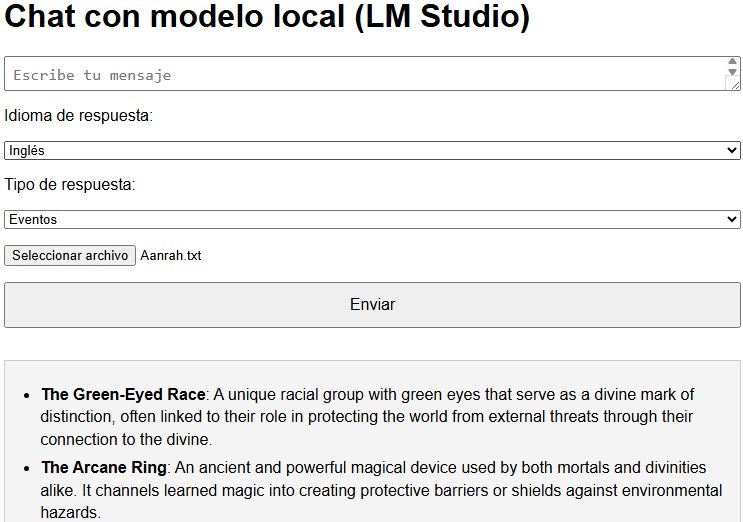
\includegraphics[width=0.85\textwidth]{./Figures/full-promp-testing.png}
	\caption{Prueba de la versión definitiva del sistema.}
	\label{fig:full-prompt-test}
\end{figure}

\subsection{Resultados de \textit{deepseek}}
Este modelo experimentó una mejora sustancial en la calidad de sus respuestas, tanto en la profundidad
contextual como en la variedad de las ideas que aporta.
La capacidad del modelo para relacionar elementos de la ambientación narrativa y
plasmarlos en las propuestas se vio significativamente potenciada, abarcando eventos, personajes y geografía
(ver figura \ref{fig:deepseek-prompt-char}).
La consistencia de las respuestas se mantuvo estable,
reduciéndose notablemente la aparición de errores de formato y temática.
Asimismo, el rendimiento en español mejoró, reduciendo el coste de la traducción.

\begin{figure}[htbp]
	\centering
	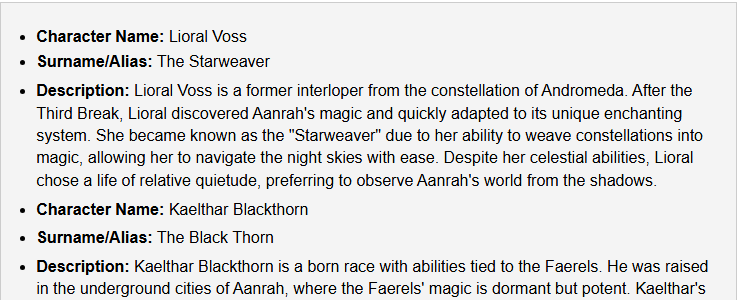
\includegraphics[width=1\textwidth]{./Figures/deepseek-prompt-characters.png}
	\caption{Resultado de \textit{deepseek} para personajes.}
	\label{fig:deepseek-prompt-char}
\end{figure}
\pagebreak
\subsection{Resultados de \textit{mistral}}
\textit{Mistral} mostró una adaptación inconsistente a la ingeniería de instrucciones precisas,
lo que se tradujo en una alta variabilidad en sus respuestas.
Aunque en algunos casos interpretó correctamente las directrices,
mostrando una ligera mejora respecto a las instrucciones básicas,
los errores fueron frecuentes. Entre los más comunes se incluyen la duplicación de la lista generada y
una pérdida considerable de la temática en la respuesta. Esto a menudo resultaba en la generación de más de los 10 elementos especificados por defecto,
con una relación mínima o nula con el contexto general.
Además, el modelo perdió por completo su capacidad de generar respuestas en español bajo esta configuración.

\begin{figure}[htbp]
	\centering
	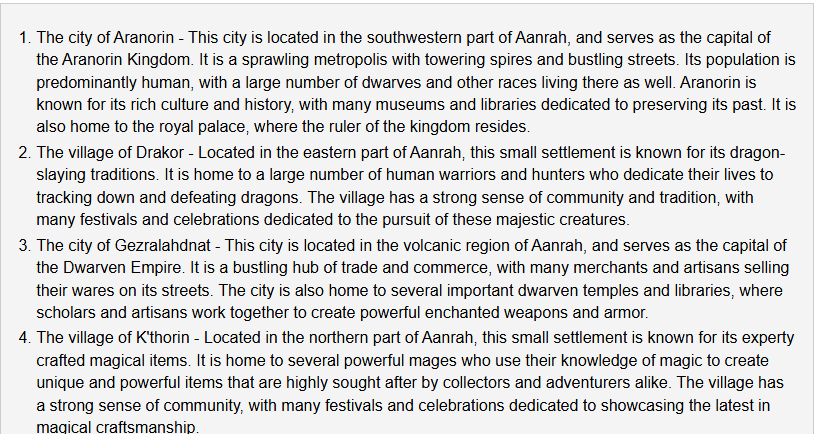
\includegraphics[width=1\textwidth]{./Figures/mistral-prompt-locations.png}
	\caption{Resultado de \textit{mistral} para localizaciones.}
	\label{fig:mistral-prompt-locations}
\end{figure}

%----------------------------------------------------------------------------------------
%	SECTION 8
%----------------------------------------------------------------------------------------
\section{Pruebas con modelos reentrenados y \textit{prompting} preciso}
Esta sección presenta y analiza los resultados obtenidos de las pruebas realizadas sobre los modelos refinados,
empleando esta vez instrucciones precisas.

\subsection{Resultados de \textit{writing-roleplay}}
La comprensión del LLM experimentó una ligera mejora,
siendo esta más evidente en la generación de eventos.
Sin embargo, en el resto de categorías, el rendimiento se mantuvo similar al observado con \textit{prompting} poco preciso.
En varias ocasiones, el modelo interpretó que debía generar una lista de varias decenas de puntos,
lo que provocó bloqueos en el sistema, indicando una posible sobrecarga o un fallo en el manejo de la longitud de la respuesta esperada.

\begin{figure}[htbp]
	\centering
	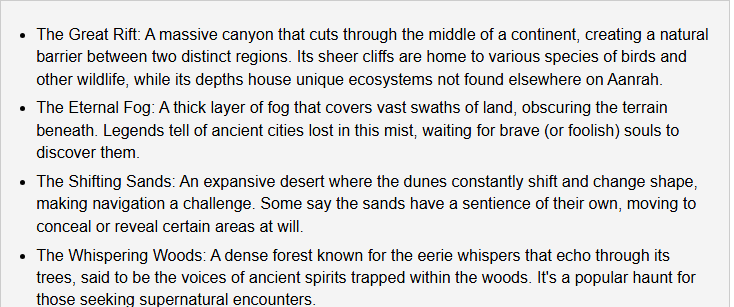
\includegraphics[width=1\textwidth]{./Figures/writing-prompt-geography.png}
	\caption{Resultado de \textit{writing-roleplay} para geografía.}
	\label{fig:writing-geography}
\end{figure}

\subsection{Resultados de \textit{worldbuilder}}
Con la aplicación de las nuevas instrucciones, el modelo mostró
una mejora perceptible en la comprensión del contexto de entrada,
lo cual se reflejó en la calidad de la generación.
No obstante, en los apartados de geografía y localizaciones, no se observó una mejora significativa.
En esta configuración, también se registraron alucinaciones, como se ilustra en la figura \ref{fig:worldbuilder-hallucination},
que complejizaron el listado y llevaron a la devolución de varias listas con diferentes categorías,
sugiriendo nuevamente una tendencia a desviarse de la estructura de respuesta esperada.

\begin{figure}[htbp]
	\centering
	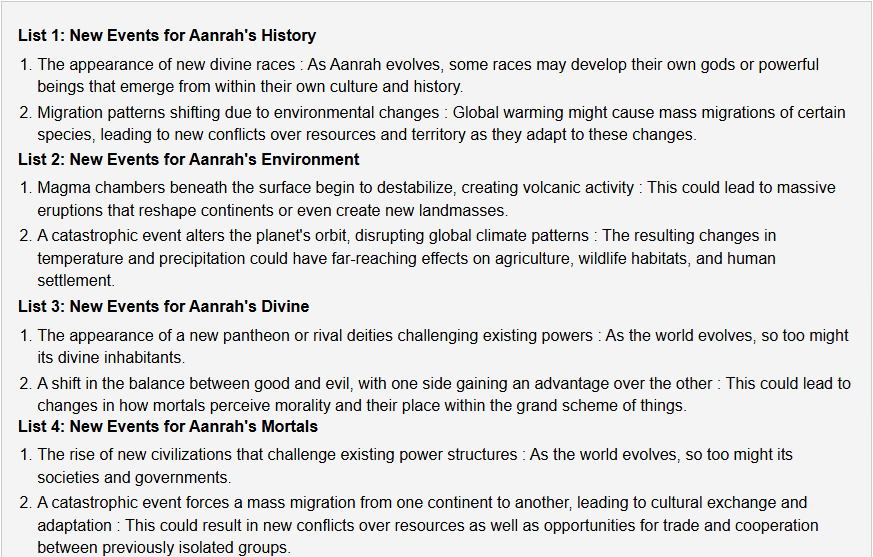
\includegraphics[width=0.8\textwidth]{./Figures/worldbuilder-hallucination-events.png}
	\caption{Alucinación de \textit{worldbuilder} en la generación de eventos.}
	\label{fig:worldbuilder-hallucination}
\end{figure}

\subsection{Resultados de \textit{arliai-rpmax}}
Gracias al refinamiento de los \textit{prompts},
este modelo mejoró significativamente su comprensión e inclusión del contexto,
lo que resultó en respuestas de calidad excepcional.
Además, \textit{arliai-rpmax} destacó por su robusta capacidad de generar texto en español,
manteniendo una calidad constante en el mensaje sin degradación.

\begin{figure}[htbp]
	\centering
	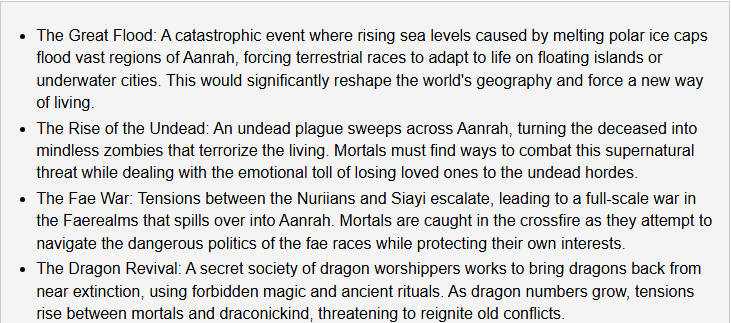
\includegraphics[width=1\textwidth]{./Figures/rpmax-prompt-events.png}
	\caption{Resultado de \textit{arliai-rpmax} en la generación de eventos.}
	\label{fig:rpmax-events}
\end{figure}

A nivel global, se observó una mejora consistente en la generación de eventos por parte de todos los LLM,
en comparación con las evaluaciones previas.
Sin embargo, los resultados no fueron tan favorables en la creación de personajes,
la geografía y las localizaciones,
donde los modelos continuaron exhibiendo limitaciones en originalidad y variedad.
Este fenómeno plantea la necesidad de investigar si se debe a un posible sobreentrenamiento en ciertas categorías
o a una escasez de información contextual relevante en la ambientación narrativa empleada en los ensayos.

%----------------------------------------------------------------------------------------
%	SECTION 9
%----------------------------------------------------------------------------------------
\section{Interpretación de resultados}
Previo al análisis global del rendimiento del sistema,
se han confeccionado dos grillas resumen que muestran cómo ha funcionado
cada combinación de modelo y estrategia de instrucciones a lo largo de la experimentación.
En ella, cada celda contiene una valoración del 1 al 5,
donde 1 indica un desempeño insuficiente y 5 refleja una ejecución excelente.
Esta síntesis numérica de las tablas \ref{tab:results-noprompt} y \ref{tab:results-prompt}
permite identificar patrones de mejora derivados
de intervenciones específicas, como la optimización de los \textit{prompts},
y facilita una evaluación comparativa entre configuraciones.
 
\begin{table}[h]
\centering
\caption{Tabla resumen de los ensayos con \textit{prompting} poco preciso.}
\resizebox{\textwidth}{!}{%
\begin{tabular}{l c c c c c c c c}
\toprule
\textbf{Modelo} & \textbf{Eventos} & \textbf{Personajes} & \textbf{Geografía} & \textbf{Localizaciones} & \textbf{Contexto} & \textbf{Temática} & \textbf{Originalidad} & \textbf{Consistencia} \\
\midrule
\texttt{deepseek} & 3 & 2 & 3 & 3 & 3 & 4 & 3 & 2 \\
\texttt{mistral} & 1 & 2 & 3 & 3 & 2 & 3 & 2 & 4 \\
\texttt{writing-roleplay} & 3 & 2 & 3 & 3 & 2 & 4 & 3 & 3 \\
\texttt{worldbuilder} & 4 & 3 & 3 & 3 & 3 & 4 & 4 & 3 \\
\texttt{arliai-rpmax} & 4 & 4 & 3 & 3 & 3 & 4 & 3 & 3 \\
\bottomrule
\end{tabular}%
}
\label{tab:results-noprompt}
\end{table}

\begin{table}[h]
\centering
\caption{Tabla resumen de los ensayos con \textit{prompting} preciso.}
\resizebox{\textwidth}{!}{%
\begin{tabular}{l c c c c c c c c}
\toprule
\textbf{Modelo} & \textbf{Eventos} & \textbf{Personajes} & \textbf{Geografía} & \textbf{Localizaciones} & \textbf{Contexto} & \textbf{Temática} & \textbf{Originalidad} & \textbf{Consistencia} \\
\midrule
\texttt{deepseek} & 4 & 3 & 4 & 3 & 4 & 3 & 4 & 3 \\
\texttt{mistral} & 2 & 2 & 3 & 3 & 3 & 3 & 3 & 2 \\
\texttt{writing-roleplay} & 4 & 3 & 2 & 2 & 3 & 3 & 3 & 2 \\
\texttt{worldbuilder} & 4 & 4 & 3 & 3 & 4 & 4 & 4 & 3 \\
\texttt{arliai-rpmax} & \textbf{5} & 4 & 3 & 3 & 4 & 4 & 4 & 4 \\
\bottomrule
\end{tabular}%
}
\label{tab:results-prompt}
\end{table}

\pagebreak
Teniendo en cuenta las puntuaciones, se pueden sacar las siguientes conclusiones:

\begin{itemize}
\item Los modelos generalistas tienen un rendimiento menor que aquellos LLM
	  que han sido reentrenados para la generación de contenido narrativo.
\item Es muy importante realizar una configuración de temperatura específica
      en cada modelo para limitar la aleatoriedad de la estructura de las respuestas.
\item Todos los modelos presentaron rigidez en la creación de algunos elementos narrativos,
	  posiblemente por requerir un mayor nivel de creatividad o por no tener suficiente contexto previo.
\item La estrategia de instrucciones desarrollada mejora notablemente la capacidad de profundizar en el
      contexto de entrada y plasmarlo en la salida, a costa de aumentar su inestabilidad en algunos casos.
\end{itemize}

Durante las pruebas se encontraron los siguientes errores con una frecuencia o gravedad considerables:
\begin{itemize}
\item Error de formato:
	  aunque no se trata de un problema con un impacto notable,
	  el formato de la salida de texto variaba en cada ejecución.
	  A veces empleaba listas de puntos, otras veces listas numeradas y, en raras ocasiones,
	  ignoró el formato y lo separó en párrafos.
	  Se estudió la posibilidad de forzar la salida de forma estructurada, pero los modelos no
	  respondieron positivamente al cambio, por lo que se concluyó que se implementará en trabajos futuros.
\item Tendencia de los LLM a generar preámbulo y resumen final:
      relacionado con el punto anterior,
	  algunos modelos tenían la tendencia de añadir información adicional alrededor de la lista de ideas.
	  En muchos de los casos, parafraseando las instrucciones recibidas por el módulo de instrucciones.
\item Errores de traducción: la mayoría de los modelos empeoraron su rendimiento al forzar su salida de 
      texto en español. Esto puede mitigarse integrando un modelo \textit{encoder} especializado en traducción
	  que actúe como etapa previa y posterior al modelo generador.
\item Procesamiento ``infinito'' de las peticiones:
	  aunque ocurrió en contadas ocasiones, este fenómeno provocaba que los modelos se quedaran
	  generando un texto demasiado largo, lo que hacía que su tiempo de respuesta aumentara
	  de unos pocos segundos a varios minutos, dando a entender que el sistema se había quedado bloqueado.
	  Este problema se puede mitigar mostrando este proceso de acumulación de palabras en tiempo real
	  o forzando su finalización tras alcanzar un tiempo o extensión configurable.
\end{itemize}
